\documentclass{standalone}
\usepackage{tikz}
\usepackage{ctex,siunitx,upgreek}
\usepackage{tkz-euclide}
\usepackage{amsmath}
\usetikzlibrary{patterns, calc}
\usetikzlibrary {decorations.pathmorphing, decorations.pathreplacing, decorations.shapes,}
\begin{document}
\small
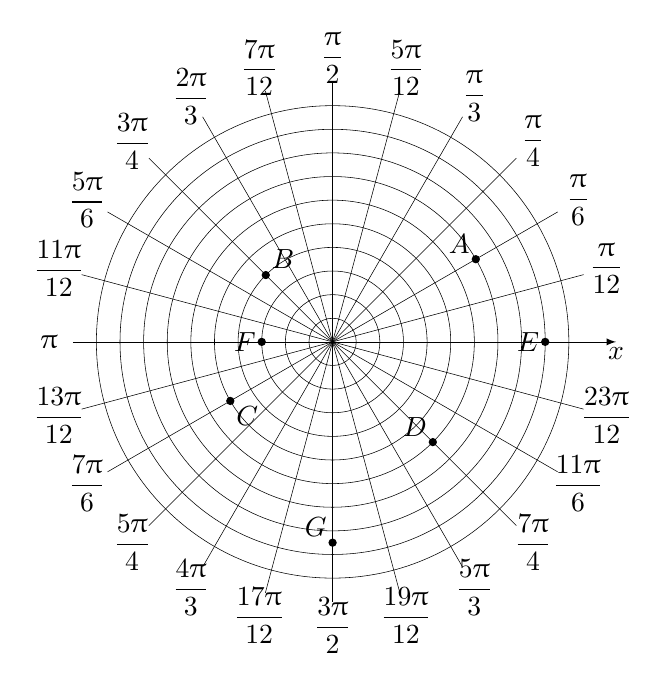
\begin{tikzpicture}[>=latex,scale=0.3,inner sep=2pt]
  \draw[very thin,->](-11,0)--(12,0)node[below]{$x$};
  \foreach \r/\a/\t/\p in {
    7/30/A/above left,
    4/135/B/above right,
    5/210/C/below right,
    6/-45/D/above left,
    9/0/E/left,
    3/180/F/left,
    8.5/-90/G/above left}
  {
    \fill(\a:\r)circle(5pt)node[\p]{$\t$};
  }
  \foreach \x in {1,...,10}
  {
    \draw[very thin](0,0)circle(\x);
  }
  \foreach \x/\a/\b in {
    15/12/{},
    30/6/{},
    45/4/{},
    60/3/{},
    75/12/5,
    90/2/{},
    105/12/7,
    120/3/2,
    135/4/3,
    150/6/5,
    165/12/11,
    % 180/12/{},
    195/12/13,
    210/6/7,
    225/4/5,
    240/3/4,
    255/12/17,
    270/2/3,
    285/12/19,
    300/3/5,
    315/4/7,
    330/6/11,
    345/12/23
  }
  {
    \draw[very thin](0,0)--(\x:11);
    \node at (\x:12) {$\dfrac{\b\uppi}{\a}$};
  }
  \node at (-12,0){$\uppi$};
\end{tikzpicture}
\end{document}